\documentclass{cheatsheet}
\usepackage{blindtext}
\usepackage{graphicx}
\usepackage{caption}


\author{ehaller, seyohnp}
\doctitle{Advanced Finance - Cheatsheet}

\begin{document}

\section*{Terminology}
    \textbf{Derivatives}: Any financial instrument that is derived from another e.g. options, warrants, futures, swaps\\
    \textbf{Option}: gives the holder the right to buy or sell a security at a specified price during a specified time period\\        \textbf{Call Option}: The right to buy a security at a specified price within a specified time\\
    \textbf{Option Premium}: The price paid for the option, above the price of the underlying security\\
    \textbf{Intrinsic Value}: Difference between the strike price and the stock price\\
    \textbf{Time Premium}: Value of option above the intrinsic value\\
    \textbf{Exercise Price}: (Strike Price) The price at which you uby or sell the security\\
    \textbf{American Option}: Can be exercised at any time prior to and including the expiration date\\
    \textbf{European Option}: Can be exercised only on the expiration date\\
    \textbf{Exercise price $\uparrow$}: \textbf{Call Price $\downarrow$}, \textbf{Put Price $\uparrow$}\\  
    \textbf{Put Option}: The right to sell a security at a specified price within a specified time\\
    \textbf{Butterfly}\\
    \textbf{Straddle}\\
    \textbf{Strategy of buying a call}: \textcolor{red}{Bild einfügen}\\
    \textbf{Value of company's assets} \textbf{$\uparrow$}, \textbf{Value of default put $\downarrow$}\\
    \textbf{Std dev asset value} \textbf{$\uparrow$}, \textbf{Value of default put $\uparrow$}\\
    \textbf{Amount of outstanding debt} \textbf{$\uparrow$}, \textbf{Value of default put $\uparrow$}\\
    \textbf{Debt maturity} \textbf{$\uparrow$}, \textbf{Value of default put $\uparrow$}\\
    \textbf{Default-free interest rate} \textbf{$\uparrow$}, \textbf{Value of default put $\downarrow$}\\
    \textbf{Dividend payments} \textbf{$\uparrow$}, \textbf{Value of default put $\uparrow$}\\
    \textbf{Indenture or trust deed}: The bond agreement between the borrower and a trust company\\
    \textbf{Registered bond}: A bond in which the company's records show ownership and interest and principal are paid directly to each owner.\\
    \textbf{Bearer bonds}: The bondholder must send in coupons to claim interest and mus send a certificate to claim the final payment of principal\\
    \textbf{Accrued interest}: The amount of accumulated interest since the last coupon payment\\
    \textbf{Coupon}: Interest paid on a bond\\
    \textbf{Debentures}: Long-term unsecured issues on debt\\
    \textbf{Mortgage bond}: Long-term secured debt, often containing a claim against a specific building or property\\
    \textbf{Collateral trust bonds}: Bonds secured by common stocks or other securities that are owned by te borrower\\
    \textbf{Equipmnet trust certificate}: Secured debt generally used to finance railroad equipment. The trustee retains equipment ownership until the debt is repaid.\\
    \textbf{Asset-backed securities}: The sale of cash flows derived directly from a specific set of bundled assets\\
    \textbf{Mortgage-backed securites}: Package of mortgage loans sold; owners of package receive portion of mortgage payments\\
    \textbf{Callable bond}: Allows the issuer to repay the debt, valuable to reduce leverage\\
    \textbf{Puttable (retractable) bond}: Allows the investor to be reapid for the debt, A protective covenant for the investor\\
    \textbf{Sinking fund}: A fund established to retire debt before maturity\\
    \textbf{Bond covenants}: Debt ratios, Security, Dividends, Event risk, (+) working capital, (+) net worth\\
    \textbf{Lease}: Rental agreement that involves fixed payments from lessee to lessor (\textit{Reasons: convenient, provided maintenance, low cost through standardization, tax shields, financial distress, avoid capital expenditure controls, preserve capital off-balance sheet financing})
    \textbf{Direct Lease}: The lessor buy the equipment from the manufacturer
    \textbf{Full Service Lease}: The lessor provides maintenance and insurance
    \textbf{Operating Lease}: The initial lease period is shorter than the economic life of the asset
    \textbf{Financial Lease}: The initial lease period is long enough for the lessor to recover the cost of the asset
    \textbf{Net Lease}: The lessee provides maintenance and insurance
    \textbf{Leveraged Lease}: The lessor finances the lease contract by issuing debt and equity claims against it
    \textbf{Sale and Leaseback}: The lessors buys the equipment from the prospective lessee
    \textbf{Spot price}: Price paid for immediate delivery
    \textbf{Forward vs futures contract}: Both contracts buy or sell at a specified future date at a specified price. However, compared to forwards, futures are traded on an exchange and they are marked to market. \textit{Futures fixes a price which has to be payed if market value is higher or lower}
    \textbf{Long vs short position}: Investors who are long have agreed to buy the asset. Investors who are short have contracted to sell.
    \textbf{Basis risk}: The risk that arises because the price of the asset used to hedge is not perfectly correlated with that of the asset that is being hedged.
    \textbf{Mark to market}:Profits and losses on a position are settled on a regular basis
    \textbf{Net convenience yield}: The advantage from owning the commodity rather than the promise of future delivery less the cost of storing the commodity
    \textbf{Exchange Rate}: Amount of one currency needed to buy one unit on another
    \textbf{Spot Rate of Exchange}: Exchange rate for an immediate transaction
    \textbf{Forward Exchange rate}: Exchange rate for a forward transaction

\section*{Formulas}
\subsection{Put-Call-Parity}
    \[
C + PV(EX) = P + S
\]

\noindent where:
\begin{itemize}
  \item $C$ = Price of the European call option
  \item $PV(EX)$ = Present value of the strike price = $\frac{Ex.Price}{(1+r)}$
  \item $P$ = Price of a European Put
  \item $S$ = Share Price
\end{itemize}
\subsection{Option $\Delta$}
\[Option \Delta = \frac{C_u - C_d}{S_u - S_d} = \frac{P_u - P_d}{S_u - S_d}\]
\noindent where:
\begin{itemize}
  \item $C_u$ = Call upside
  \item $C_d$ = Call downside
  \item $P$ = Put
  \item $S$ = Stock
\end{itemize}
\subsection{Risk neutral probability of rising value}
\[p^{*} = \frac{(1+r) - d}{u-d}\]
\noindent where:
\begin{itemize}
  \item $r$ = Interest rate
  \item $d$ = Relative downward change
  \item $u$ = Relative upward change
\end{itemize}
\subsection{Expected Value}
\[Expected Value = (p^{*} * PayOff_u) + ([1 - p^{*}] * PayOff_d)\]
\subsection{Present Value}
\[Present Value = \frac{Expected Value}{(1+r)} = ValueShares - ValueLoan\]
\[Value Loan = \frac{ValueShares_d}{(1+r)}\]
\subsection{Up and Down Changes}
\[1 + UpsideChange = u = e^{\sigma*\sqrt{h}}\]
\[1 + DownsideChange = d = \frac{1}{u}\]
\noindent where:
\begin{itemize}
  \item $\sigma$ = Standard Deviation
  \item $h$ = Fraction of Year
\end{itemize}
\subsection{Black-Scholes Formula(weg wenn zu viel)}
\[C = (N[d_1] * S) - (N[d_2] * PV[EX])\]
\[d_1 = \frac{log(\frac{S}{PV[EX]})}{\sigma *\sqrt{t}} + \frac{\sigma\sqrt{2}}{2}\]
\[d_2 = d_1 - \sigma\sqrt{t}\]
\noindent where:
\begin{itemize}
  \item $C$ = Call Value
  \item $N[d]$ = Cummulative normal probability
  \item $PV(EX)$ = Ex. Price at risk-free interest rate
  \item $S$ = Stock price
  \item $t$ = number of periods tp exercise date
  \item $\sigma$ = Standard Deviation 
  \item $if d_1 is large, N(d_1) is close to 1.0$
  \item $if d_1 is zero, N(d_1) is close to 0.5$
\end{itemize}
\subsection{Present Value Formlua BOND}
\[PV = \sum_{t=1}^{T}\frac{cpn}{(1+r)^{t}}+\frac{par}{(1+r)^{T}}\]
\[Promised Yield = \frac{Payoff}{PV} - 1\]
\noindent where:
\begin{itemize}
  \item $cpn$ = Coupon rate
  \item $r$ = Interest rate
  \item $T$ = Number of periods
  \item $par$ = Face value
\end{itemize}

\subsection{Predicting Default: Altman's Z-score}
\[Z = 1.2x_1 + 1.4x_2 + 3.3x_3 + 0.6x_4 + 1.0x_5\]
\noindent where:
\begin{itemize}
  \item $x_1$ = working capital/total assets
  \item $x_2$ = retained earnings/total assets
  \item $x_3$ = earnings before interest and tax (EBIT)/total assets
  \item $x_4$ = market value of equity / total liabilities
  \item $x_5$ = sales/total assets
\end{itemize}
\subsection{Convertible Securities}
\[Conversion Price = \frac{Face Value (1000\$)}{Conversion Ratio}\]
\[Conversion Value = Conversion ratio * share price\]
\section{Take or Die}
\textbf{Expansion Options}: Uncertainty $\uparrow$ - Valoue of exp. option $\uparrow$
\textbf{Value of a call (takeaways)}: 
\begin{itemize}
  \item Never worth more than the stock price itself.
  \item When the share is worthless, the option is worthless.
\end{itemize}
\section*{Lease or Buy}
\begin{itemize}
  \item Buy if equivalent annual cost of ownership and operation is less than the best lease rate
  \item For using extended periods, buying tends to be cheaper
  \item Leasing, because lessor might be able to manage asset at less expense than lessee
  \item Leasing has useful options in leasing agreement
\end{itemize}
\[NPV_{lease} = InitialFinancing - \sum_{t=1}^{T}\frac{LeaseCashFlow}{[1 + r_D * (1-T_c)]^t}\]
\[NPV = PV_{EquivalentLoan} + InitialFinancing\]
\begin{itemize}
  \item $r_D$ = discount rate
  \item $t_c$ = marginal tax rate
\end{itemize}
\section*{Managing Risks}
\textbf{Risks to a business:} Cash shortfalls, Financial distress, Agency costs, Currency fluctuations, Political instability, Weather changes
\section*{Pricing Futures Contracts}
\[F_t = S_0 * (1 + r_f - y)^t \]
\[= S_0 * (1 + StorageCost - CY)^t\]
\[NCY = ConvenienceYield - StorageCost\]
\begin{itemize}
  \item $F_t$ = future price on contract of $t$ length
  \item $S_0$ = today's spot price
  \item $r_f$ = risk-free interest rate
  \item $y$ = dividend yield 
  \item $NCY$ = NetConvenienceYield
\end{itemize}
\section*{Hedging Rations and Basis Risk}
\[ExpectedChangeInValueA = \alpha + \delta * (ChangInValueB)\]
\begin{itemize}
  \item $\delta$ = sensitivity of A to change in the value of B (hedge ration)
  \item $\alpha$ = offset
\end{itemize}
\section*{Premium- Discount Relationship}
\[ForwardDiscount = \frac{1}{t_{years}} * (\frac{SpotPrice}{ForwardRate} - 1)\]
\section{Basic Relationships
in the FX Market}
\begin{figure}[h!]
    \centering
    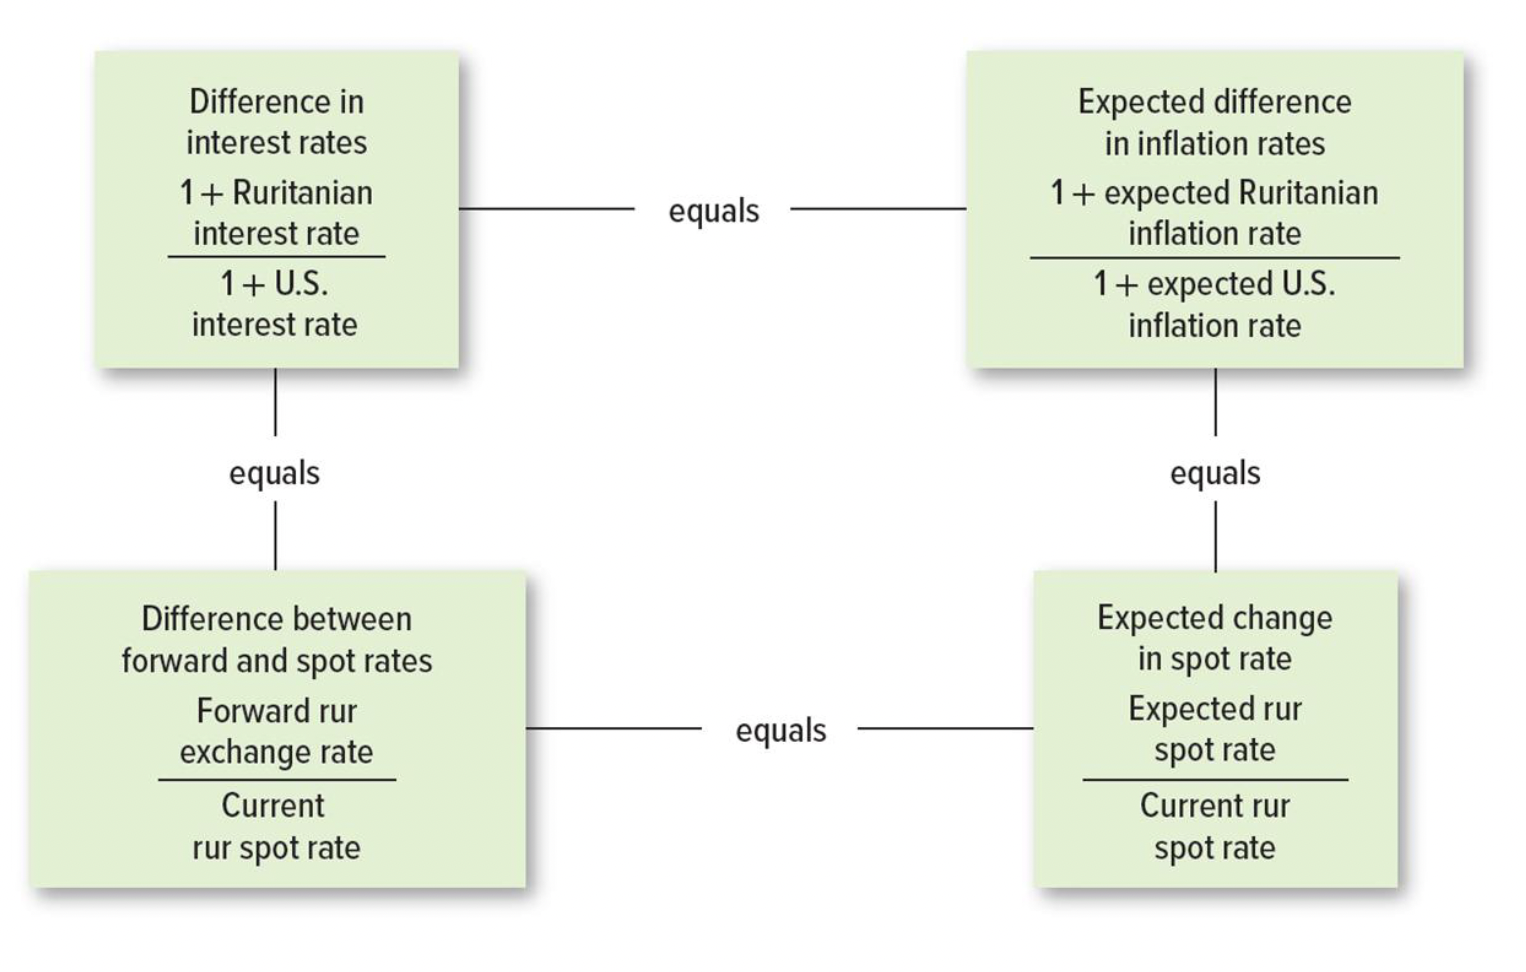
\includegraphics[width=0.2\linewidth]{Bildschirmfoto 2025-05-23 um 10.16.13.png}
    \caption{Relationship between interest rates, inflation, and exchange rates}
    \label{fig:interest_inflation_exchange}
\end{figure}
\section*{Binomial Method}
\end{document}